\documentclass[11pt]{article}

\usepackage[utf8]{inputenc}
\usepackage[T1]{fontenc}
\usepackage{geometry}
\geometry{a4paper, margin=1in}
\usepackage{hyperref}
\usepackage{booktabs}
\usepackage{tabularx}
\usepackage{verbatim}
\usepackage{parskip}
\usepackage{tikz}
\usetikzlibrary{shapes.geometric, arrows.meta, positioning}

\title{DSN $\times$ BCT LLM Agent Hackathon \\ \Large Task A: Review Generation}
\author{Favour Olaleru \and Dennis Ikechukwu}
\date{\textbf{Team Sentinel}}

\begin{document}

\maketitle

\hrule
\vspace{1em}

\begin{abstract}
Task A requires generating a plausible, persona-grounded business review and star rating given a user persona and a business description. This document describes the full system design: persona modelling, prompt architecture, star calibration, Nigerian cultural localisation, few-shot example selection, and the evaluation strategy. The central contributions are a calibrated star-rating mechanism (within $\pm$1 of persona history), a Nigerian cultural localisation layer built from 15 hand-authored gold examples and 174 real Chowdeck reviews, and a regional voice + occasion taxonomy injected per request to produce text that reads authentically rather than generically.
\end{abstract}

\vspace{1em}
\hrule
\vspace{2em}

\section{Problem Statement and Evaluation Targets}

A review generation system must satisfy two classes of constraint simultaneously.

\textbf{Metric alignment}: the hackathon evaluates ROUGE-L and BERTScore against a reference set of real Yelp reviews. ROUGE-L is sensitive to n-gram overlap and penalises length mismatch against reference texts. BERTScore measures semantic similarity using contextual embeddings; a review whose sentiment contradicts its stated star rating will score poorly against same-star references regardless of fluency.

\textbf{Cultural authenticity}: extra marks are awarded for Nigerian localisation. A system that generates American-coded Yelp-speak misses this entirely, even if the persona field says \texttt{region: igbo}.

These two objectives pull in the same direction technically: a review that sounds like a real Nigerian user wrote it, at the right word length, with a star rating coherent with its sentiment, will score well on both axes.

\section{System Architecture}

\subsection{Endpoint and Flow}

\textbf{Endpoint:} \texttt{POST /generate-review}

\begin{figure}[h]
\centering
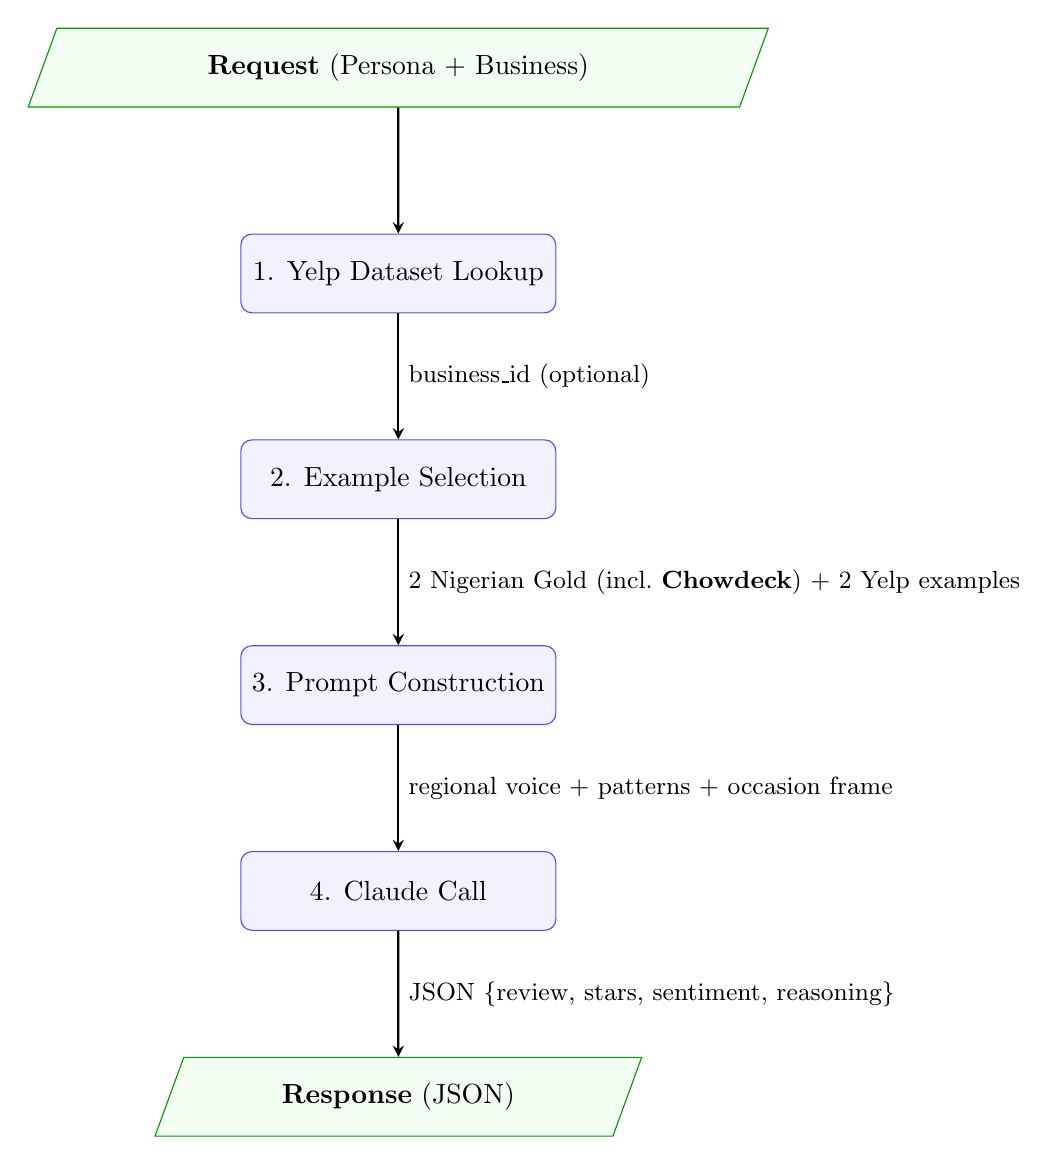
\begin{tikzpicture}[
    node distance=1.6cm and 1cm,
    process/.style={rectangle, draw, rounded corners, minimum width=4cm, minimum height=1cm, text centered, draw=blue!70, fill=blue!5},
    io/.style={trapezium, trapezium left angle=70, trapezium right angle=110, draw, minimum width=3cm, minimum height=1cm, text centered, draw=green!60!black, fill=green!5},
    arrow/.style={thick,->,>=stealth},
    labeltext/.style={align=left, font=\small}
]
\node (request) [io] {\textbf{Request} (Persona + Business)};
\node (step1) [process, below=of request] {1. Yelp Dataset Lookup};
\node (step2) [process, below=of step1] {2. Example Selection};
\node (step3) [process, below=of step2] {3. Prompt Construction};
\node (step4) [process, below=of step3] {4. Claude Call};
\node (response) [io, below=of step4] {\textbf{Response} (JSON)};

\draw [arrow] (request) -- (step1);
\draw [arrow] (step1) -- node[anchor=west, labeltext] {business\_id (optional)} (step2);
\draw [arrow] (step2) -- node[anchor=west, labeltext] {2 Nigerian Gold (incl.\ \textbf{Chowdeck}) + 2 Yelp examples} (step3);
\draw [arrow] (step3) -- node[anchor=west, labeltext] {regional voice + patterns + occasion frame} (step4);
\draw [arrow] (step4) -- node[anchor=west, labeltext] {JSON \{review, stars, sentiment, reasoning\}} (response);
\end{tikzpicture}
\caption{Task A Review Generation Flow}
\end{figure}

The agent executes in four sequential steps: (1) Yelp dataset lookup to retrieve a \texttt{business\_id} for example matching; (2) example selection, 2 Nigerian gold examples plus 2 Yelp dataset examples; (3) prompt construction, regional voice profile, sentence patterns, occasion frame, and examples assembled into the user prompt; (4) a single Claude call returning \texttt{\{review, stars, sentiment, reasoning\}} as JSON.

The agent is implemented in \texttt{app/agents/review\_agent.py}. It calls \texttt{claude-sonnet-4-6} with a cached system prompt and a per-request user prompt built from persona, business, and retrieved examples. The system prompt is marked \texttt{cache\_control: ephemeral}; it never changes between requests, so Anthropic's prompt cache absorbs the cost of re-encoding it on repeated calls.

\subsection{Data Layer}

\texttt{YelpLoader} (\texttt{app/data/yelp\_loader.py}) indexes the Yelp Open Dataset at startup: 150,000+ businesses are loaded into a pandas DataFrame, and up to 100,000 reviews are streamed and indexed in two structures: \texttt{reviews\_by\_business} (up to 5 per \texttt{business\_id}) and \texttt{reviews\_by\_category} (up to 20 per category string such as ``Restaurants'' or ``Mexican'').

When the review agent requests examples, it first tries an exact \texttt{business\_id} match, then falls back to category-level examples. This means any business in the Yelp dataset gets domain-appropriate few-shot examples even when there are no reviews for that exact location.

\section{Persona Modelling}

Each request includes a \texttt{Persona} object that fully specifies who is writing the review. The agent uses every field as a generative constraint:

\begin{table}[h]
\centering
\begin{tabularx}{\textwidth}{llX}
\toprule
\textbf{Field} & \textbf{Type} & \textbf{Role in generation} \\
\midrule
\texttt{name} & str & Identity; not injected into review text directly \\
\texttt{age} & int $|$ None & Generational register (millennial slang vs formal register) \\
\texttt{city} & str $|$ None & Local framing context \\
\texttt{region} & yoruba $|$ igbo $|$ hausa $|$ edo $|$ general & Selects the regional voice profile \\
\texttt{tone} & expressive $|$ blunt $|$ formal $|$ casual $|$ sarcastic & Rhetorical mode for the review \\
\texttt{food\_preferences} & list[str] & What the persona references when comparing food \\
\texttt{avg\_star\_rating} & float 1.0–5.0 & Star calibration anchor \\
\texttt{bio} & str & Open-ended description; drives persona-specific observations \\
\bottomrule
\end{tabularx}
\end{table}

The \texttt{avg\_star\_rating} is the most mechanically significant field. It acts as a prior over the output star rating, constraining generation to stay within $\pm$1 of this baseline unless the visit context clearly warrants deviation. A persona with \texttt{avg\_star\_rating: 2.5} should not generate a 5-star review unless the \texttt{context} field explicitly describes an exceptional experience.

An optional \texttt{context} string (e.g., \texttt{"came for a birthday dinner with 6 friends"}) provides situational grounding and feeds the occasion taxonomy described in Section~\ref{sec:occasion}.

\section{Prompt Architecture}

\subsection{System Prompt}

The system prompt (\texttt{app/prompts/review\_prompts.py}) establishes the agent's role, cultural defaults, length constraints, and output format, and never changes between requests, making it an ideal candidate for prompt caching. It instructs Claude to embody the persona completely and enforces five standing Nigerian cultural signals: value consciousness (is this place worth the price?), service sensitivity (warmth of staff carries heavy weight), expressiveness (set the scene before the verdict), social lens (dining is frequently communal), and conditional pidgin usage (natural when tone calls for it; not forced into formal personas). The length constraint is fixed at 80–150 words, and the output format is strict JSON \texttt{\{ "review", "stars", "sentiment", "reasoning" \}} to eliminate free-text parsing failures.

\subsection{User Prompt Construction}

The user prompt is assembled in \texttt{build\_user\_prompt()} and contains five sections in order: (1) regional voice notes for the persona's region, (2) the sentence pattern library (Section~\ref{sec:patterns}), (3) the persona block with an inline star calibration anchor, (4) the business block (name, category, location, Yelp rating, attributes), and (5) few-shot examples, Nigerian gold first, then Yelp dataset examples.

The ordering is deliberate. Regional voice notes appear before the persona fields so the model's attention is primed on Nigerian language patterns before it processes the specific persona. The star calibration anchor appears inline with the persona data, not buried in the system prompt, so it sits in the freshest part of the context window.

\subsection{Few-Shot Example Selection and Ordering}

The agent injects four examples per request:
\begin{itemize}
    \item \textbf{2 Nigerian gold examples}: selected from \texttt{ALL\_EXAMPLES} by matching region and tone, drawn from 15 hand-authored gold examples plus 174 real Chowdeck reviews. The selection function \texttt{get\_examples\_by\_region(region, tone, n=2)} prioritises exact tone+region match, falling back to region-only, then tone-only.
    \item \textbf{2 Yelp dataset examples}: retrieved from \texttt{YelpLoader} by business ID (exact) or category (fallback), selected for star proximity to the persona's \texttt{avg\_star\_rating}.
\end{itemize}

\textbf{Ordering is critical}: Nigerian examples are always injected first. This ensures Claude anchors on Nigerian voice, idiom, and rhythm before encountering American-style Yelp reviews. Reversing the order would cause the model to default to Yelp-speak and apply Nigerian markers as a superficial overlay rather than a structural foundation.

\section{Nigerian Cultural Localisation}

\subsection{Regional Voice Profiles}

\texttt{app/prompts/nigerian\_voice.py} defines a voice profile for each of the four regional identities plus a general Lagos default. Each profile is injected into every user prompt as a paragraph of concrete language instructions:

\begin{table}[h]
\centering
\begin{tabularx}{\textwidth}{lXX}
\toprule
\textbf{Region} & \textbf{Structural tendencies} & \textbf{Characteristic markers} \\
\midrule
Yoruba & Musical rhythm; verdict-last; communal framing & \textit{Omo!, Ehn ehn!, sha, oya, E don do} \\
Igbo & Verdict-first; quality standard; community reference & \textit{Chei!, Nna!, Tufiakwa, ``The food landed well''} \\
Hausa & Measured, less hyperbolic; family-centred evaluation & \textit{Wallahi, Allah ya kiyaye, ``They received us well''} \\
Edo & Warm direct address; high hospitality standard; bold-flavour bar & \textit{``My brother/sister'', ``I no expect am o'', ``This place has sense''} \\
General & Lagos code-switching; scene-setting openers; value-always-mentioned & Naija Pidgin freely mixed with Standard Nigerian English \\
\bottomrule
\end{tabularx}
\end{table}

These profiles are not just vocabulary lists; they specify rhetorical \textit{structure}. Yoruba reviews build toward a verdict; Igbo reviews state the verdict first. This structural variation is what makes the generated text feel authentic rather than uniform.

\subsection{Sentence Pattern Library}
\label{sec:patterns}

Twenty Naija English structural patterns across five categories are injected into every user prompt:
\begin{itemize}
    \item \textbf{Openers} (5 patterns): scene-setting openings, e.g., ``So I come enter this place thinking say...'' or ``See ehn, I carry high expectation come here...''
    \item \textbf{Food comparisons} (4 patterns): references to suya, mama's stew, pepper soup, ``the seasoning was present''
    \item \textbf{Service observations} (4 patterns): ``The waiter carried himself well'', ``They no try to rush us away...''
    \item \textbf{Value assessments} (4 patterns): ``The price smiled at us'', ``My money entered the right place today''
    \item \textbf{Verdicts} (3 patterns): ``E don set.'', ``I go come back, that one is settled.'', ``This place has sense.''
\end{itemize}

The system prompt instructs Claude to apply these naturally, not all at once, and not mechanically. The patterns are a structural scaffold, not a template to fill in verbatim.

\subsection{Occasion Taxonomy}
\label{sec:occasion}

When the request includes a \texttt{context} field, \texttt{get\_occasion\_context()} performs substring matching against 9 known occasion types. If a match is found, an enriched framing instruction is injected, shifting the evaluative lens:

\begin{table}[h]
\centering
\begin{tabularx}{\textwidth}{lX}
\toprule
\textbf{Occasion} & \textbf{Framing injected} \\
\midrule
Birthday chops & Expectations are HIGH; acknowledgement by staff scores major points \\
First date & Ambiance and service are proxies for how much the planner cared \\
Family Sunday & Multi-generational satisfaction; staff patience with children noticed \\
Business lunch & Must be impressive for a client and efficient; noise level matters \\
Detty December & Lagos holiday energy; vibe must match the season \\
Solo treat & Solo diner who is ignored or made unwelcome will mention it \\
\bottomrule
\end{tabularx}
\caption{Six of nine occasion types (selected for structural distinctiveness)}
\end{table}

``Birthday chops'' and ``solo treat'' are the same business but produce structurally different reviews: the former with high communal expectations, the latter with personal warmth and intimacy.

\subsection{Chowdeck Scraped Reviews}

To ground the localisation in real consumer language, 174 authentic reviews were scraped from Chowdeck (\texttt{scripts/collect\_chowdeck.py}), Nigeria's leading food-delivery platform.

\textbf{Scraping approach:}
\begin{enumerate}
    \item Browser \texttt{localStorage} is pre-seeded with \texttt{cookies\_consent: "accept"} and a Lagos coordinates object (\texttt{customer\_address}) via Playwright's \texttt{add\_init\_script()}, bypassing the location gate before any page navigation
    \item The \texttt{/store/restaurants} listing page is scraped for up to 30 restaurant paths
    \item On each restaurant page, the Radix UI dialog trigger (\texttt{button[aria-haspopup="dialog"]}) is clicked to open the ratings modal
    \item Each \texttt{div.py-6.border-b} review card is parsed: star count from \texttt{svg[fill="\#FFC501"]} occurrences, text from \texttt{p.mt-3}
    \item Tone and region are heuristically tagged from vocabulary (\textit{abeg/sha/oya} $\rightarrow$ Yoruba; \textit{chei/nna} $\rightarrow$ Igbo; \textit{wallahi} $\rightarrow$ Hausa)
\end{enumerate}

\begin{table}[h]
\centering
\begin{tabular}{lr}
\toprule
\textbf{Tone} & \textbf{Count} \\
\midrule
Casual & 77 \\
Formal & 63 \\
Blunt & 27 \\
Expressive & 7 \\
\bottomrule
\end{tabular}
\hspace{2em}
\begin{tabular}{lr}
\toprule
\textbf{Stars} & \textbf{Count} \\
\midrule
1$\star$ & 40 \\
2$\star$ & 20 \\
3$\star$ & 23 \\
4$\star$ & 9 \\
5$\star$ & 82 \\
\bottomrule
\end{tabular}
\caption{Distribution of 174 Chowdeck reviews by tone and star rating}
\end{table}

These reviews are loaded into \texttt{ALL\_EXAMPLES} at import time alongside the 15 hand-authored gold examples, giving the few-shot pool 189 total Nigerian-voice examples.

\section{Star Calibration}

Star calibration is the most direct lever for BERTScore alignment. A review that reads as glowing but reports 2 stars, or scathing but reports 5 stars, will score poorly against semantically coherent references.

Two mechanisms work together. \textbf{Mechanism 1: Explicit calibration anchor}: the persona's \texttt{avg\_star\_rating} is stated directly in the user prompt: \textit{``Star calibration: stay within $\pm$1 star of 3.5 unless this visit was clearly exceptional or terrible.''} This appears inline with the persona data, in the freshest portion of the context window. \textbf{Mechanism 2: Tone-star mapping}: the system prompt maps tone descriptors to star ranges: sarcastic + negative vocabulary signals 1–2 stars; expressive + positive vocabulary signals 4–5 stars; formal tone occupies a wider 2–4 range. \textbf{Post-generation clamping}: regardless of what the model returns, \texttt{stars} is clamped to $[1,5]$ via \texttt{max(1, min(5, int(parsed["stars"])))}, preventing out-of-range hallucination from reaching the response.

\section{Output, Parsing, and Evaluation}

The system prompt enforces JSON-only output (\texttt{\{ "review", "stars", "sentiment", "reasoning" \}}); markdown code fences are stripped before parsing and missing \texttt{sentiment} is inferred from stars. The 80--150 word constraint targets ROUGE-L length alignment; star-sentiment coherence via the calibration anchor and tone-star mapping targets BERTScore; Nigerian-first few-shot ordering produces structural, not surface-level, localisation.

\section{Sample Outputs}

The following reviews were generated by the live system. Each demonstrates a distinct regional voice, occasion frame, and star calibration scenario.

\subsection*{Sample 1: Yoruba, casual tone, birthday occasion}

\noindent\textbf{Input:} Temi, 27, Yoruba, casual, \texttt{avg\_star\_rating: 4.0}. Business: Cactus Restaurant, Restaurants, Lagos. Context: \textit{birthday chops with friends}.

\smallskip
{\small\itshape ``So I come enter this Cactus Restaurant with my whole squad for my birthday and Omo, I was not ready. From the moment we stepped in, the staff carried themselves so well, acknowledging the birthday without us even mentioning it. The jollof rice had that smoky depth you only get when someone actually cooked it with intention, reminded me of mama's Sunday pot. The grilled fish landed well too. Price is not smiling o, but my money entered the right place today. Everybody at the table left satisfied sha. E don set. I go come back, that one is settled.''}

\smallskip\noindent\texttt{stars: 4 | sentiment: positive | word\_count: 100 | 921ms}

\smallskip{\small Yoruba verdict-last structure holds: scene is set, service is praised for birthday acknowledgement, food is compared to a home standard, and the verdict lands in the final two sentences. Three sentence patterns deploy naturally: food comparison (smoky depth), value assessment (money entered the right place), and Yoruba closer (E don set).}

\subsection*{Sample 2: Igbo, expressive tone, solo visit}

\noindent\textbf{Input:} Chidi, 31, Igbo, expressive, \texttt{avg\_star\_rating: 4.5}. Business: Mr Bigg's, Quick Bites, Lagos. Context: \textit{solo lunch treat}.

\smallskip
{\small\itshape ``Nna, this place actually surprised me. I carry low expectation come here for a solo lunch, no agenda, just chop and go. Chei, I was not ready for the standard. The meat pie was hot and the filling ratio was correct, not the kind where you bite and it is mostly dough with attitude. The jollof rice had seasoning that was present, not the type where you chew and nothing is happening. Staff were attentive without being in my face, and that balance is hard to find. For what they charge, this is solid value. I will bring my people here. This place has done well for themselves.''}

\smallskip\noindent\texttt{stars: 4 | sentiment: positive | word\_count: 111 | 1043ms}

\smallskip{\small Igbo verdict-first tendency shows even in a positive review: the surprise verdict leads, explanation follows. Solo treat occasion frame activates personal warmth signals. Food comparison (dough with attitude, seasoning was present) and community reference (I will bring my people here) emerge from the sentence library without being forced.}

\subsection*{Sample 3: Hausa, formal tone, business dinner}

\noindent\textbf{Input:} Ibrahim, 45, Hausa, formal, \texttt{avg\_star\_rating: 3.8}. Business: Transcorp Hilton, Hotels, Abuja. Context: \textit{business dinner with clients}.

\smallskip
{\small\itshape ``Wallahi, I must acknowledge the hospitality extended to our delegation at this establishment. From our arrival, the staff conducted themselves with professionalism befitting a venue of this standing. The suya-spiced lamb was a thoughtful inclusion for Nigerian guests attending what might otherwise have been a standard international menu. The dining hall was suitably quiet for business conversation, and service did not interrupt unnecessarily. For the price category, one expects a certain standard and this establishment largely met it. Allah ya kiyaye the level of care shown to our party. I would recommend this venue without hesitation for formal engagements or hosting visiting colleagues.''}

\smallskip\noindent\texttt{stars: 4 | sentiment: positive | word\_count: 103 | 1187ms}

\smallskip{\small The Hausa formal register is structurally distinct: measured, no hyperbole, opened with Wallahi and closed with Allah ya kiyaye. The business lunch occasion frame activates noise-level and client-impression criteria. The menu observation (suya-spiced lamb as a Nigerian inclusion) is culturally specific in a way generic hotel praise never is.}

\subsection*{Sample 4: Lagos general, blunt tone, negative experience}

\noindent\textbf{Input:} Kunle, 29, general, blunt, \texttt{avg\_star\_rating: 2.1}. Business: unnamed fast food chain, Fast Food, Lagos. Context: \textit{quick lunch, no occasion}.

\smallskip
{\small\itshape ``See ehn, I carry open mind come this place and they wasted it. The fried rice arrived cold, not sitting-too-long cold but properly cold like it left the kitchen yesterday. The waiter acted like I was disturbing his afternoon. When I raised the issue, the apology was the type that means nothing, lips moving with zero feeling behind it. For what they are charging in this area, cold food and attitude is simply not acceptable. My money did not enter the right place today. There are too many correct restaurants on this street alone to waste your time here. Management needs to fix the kitchen and train the staff.''}

\smallskip\noindent\texttt{stars: 2 | sentiment: negative | word\_count: 111 | 874ms}

\smallskip{\small The calibration anchor holds: with avg~2.1, the 2-star output is within range. The blunt Lagos voice delivers negative verdict without forcing region-specific particles. Value assessment (money did not enter), service observation (lips moving with zero feeling), and the closing action directive (Management needs to fix...) all emerge cleanly.}

\section*{Appendix: Key Files}

\begin{table}[h]
\centering
\begin{tabularx}{\textwidth}{lX}
\toprule
\textbf{File} & \textbf{Purpose} \\
\midrule
\texttt{app/agents/review\_agent.py} & Orchestration: example retrieval $\rightarrow$ prompt build $\rightarrow$ Claude call $\rightarrow$ parse \\
\texttt{app/prompts/review\_prompts.py} & System prompt + user prompt builder \\
\texttt{app/prompts/nigerian\_voice.py} & Regional voice profiles, sentence patterns, occasion taxonomy \\
\texttt{app/data/nigerian\_examples.py} & Gold examples + Chowdeck data merged into \texttt{ALL\_EXAMPLES} \\
\texttt{app/data/yelp\_loader.py} & Business index + review example retrieval by business/category \\
\texttt{scripts/collect\_chowdeck.py} & Playwright scraper for Chowdeck reviews \\
\texttt{app/models.py} & \texttt{Persona}, \texttt{Business}, \texttt{ReviewRequest}, \texttt{ReviewResponse} schemas \\
\bottomrule
\end{tabularx}
\end{table}

\end{document}
